%%%%%%%%%%%%%%%%%%%%%%%%%%%%%%%%%%%%%%%%%
% Programming/Coding Assignment
% LaTeX Template
%
% This template has been downloaded from:
% http://www.latextemplates.com
%
% Original author:
% Ted Pavlic (http://www.tedpavlic.com)
%
% Note:
% The \lipsum[#] commands throughout this template generate dummy text
% to fill the template out. These commands should all be removed when 
% writing assignment content.
%
% This template uses a Perl script as an example snippet of code, most other
% languages are also usable. Configure them in the "CODE INCLUSION 
% CONFIGURATION" section.
%
%%%%%%%%%%%%%%%%%%%%%%%%%%%%%%%%%%%%%%%%%

%----------------------------------------------------------------------------------------
%	PACKAGES AND OTHER DOCUMENT CONFIGURATIONS
%----------------------------------------------------------------------------------------

\documentclass{article}

\usepackage{fancyhdr} % Required for custom headers
\usepackage{lastpage} % Required to determine the last page for the footer
\usepackage{extramarks} % Required for headers and footers
\usepackage[usenames,dvipsnames]{color} % Required for custom colors
\usepackage{graphicx} % Required to insert images
\usepackage{listings} % Required for insertion of code
\usepackage{courier} % Required for the courier font
\usepackage{lipsum} % Used for inserting dummy 'Lorem ipsum' text into the template
\usepackage{hyperref}

% Margins
\topmargin=-0.45in
\evensidemargin=0in
\oddsidemargin=0in
\textwidth=6.5in
\textheight=9.0in
\headsep=0.25in

\linespread{1.1} % Line spacing

% Set up the header and footer
\pagestyle{fancy}
\lhead{\hmwkAuthorName} % Top left header
\chead{\hmwkClass} % Top center head
\rhead{\firstxmark} % Top right header
\lfoot{\lastxmark} % Bottom left footer
\cfoot{} % Bottom center footer
\rfoot{Page\ \thepage\ of\ \protect\pageref{LastPage}} % Bottom right footer
\renewcommand\headrulewidth{0.4pt} % Size of the header rule
\renewcommand\footrulewidth{0.4pt} % Size of the footer rule

\setlength\parindent{0pt} % Removes all indentation from paragraphs
\setlength{\parskip}{6pt} % Add a little space between paragraphs

%----------------------------------------------------------------------------------------
%	CODE INCLUSION CONFIGURATION
%----------------------------------------------------------------------------------------

\definecolor{MyDarkGreen}{rgb}{0.0,0.4,0.0} % This is the color used for comments
\lstloadlanguages{bash} % Load Bash syntax for listings, for a list of other languages supported see: ftp://ftp.tex.ac.uk/tex-archive/macros/latex/contrib/listings/listings.pdf
\lstset{language=bash, % Use Perl in this example
        frame=single, % Single frame around code
        basicstyle=\small\ttfamily, % Use small true type font
        keywordstyle=[1]\color{Blue}\bf, % Perl functions bold and blue
        keywordstyle=[2]\color{Purple}, % Perl function arguments purple
        keywordstyle=[3]\color{Blue}\underbar, % Custom functions underlined and blue
        identifierstyle=, % Nothing special about identifiers                                         
        commentstyle=\usefont{T1}{pcr}{m}{sl}\color{MyDarkGreen}\small, % Comments small dark green courier font
        stringstyle=\color{Purple}, % Strings are purple
        showstringspaces=false, % Don't put marks in string spaces
        tabsize=5, % 5 spaces per tab
        %
        % Put standard Perl functions not included in the default language here
        morekeywords={rand},
        %
        % Put Perl function parameters here
        morekeywords=[2]{on, off, interp},
        %
        % Put user defined functions here
        morekeywords=[3]{test},
       	%
        morecomment=[l][\color{Blue}]{...}, % Line continuation (...) like blue comment
        numbers=left, % Line numbers on left
        firstnumber=1, % Line numbers start with line 1
        numberstyle=\tiny\color{Blue}, % Line numbers are blue and small
        stepnumber=5 % Line numbers go in steps of 5
}


% Creates a new command to include a perl script, the first parameter is the filename of the script (without .pl), the second parameter is the caption
\newcommand{\bashscript}[2]{
\begin{itemize}
\item[]\lstinputlisting[caption=#2,label=#1]{#1.sh}
\end{itemize}
}

%----------------------------------------------------------------------------------------
%	DOCUMENT STRUCTURE COMMANDS
%	Skip this unless you know what you're doing
%----------------------------------------------------------------------------------------

% Header and footer for when a page split occurs within a problem environment
\newcommand{\enterProblemHeader}[1]{
\nobreak\extramarks{#1}{#1 continued on next page\ldots}\nobreak
\nobreak\extramarks{#1 (continued)}{#1 continued on next page\ldots}\nobreak
}

% Header and footer for when a page split occurs between problem environments
\newcommand{\exitProblemHeader}[1]{
\nobreak\extramarks{#1 (continued)}{#1 continued on next page\ldots}\nobreak
\nobreak\extramarks{#1}{}\nobreak
}

\setcounter{secnumdepth}{0} % Removes default section numbers
\newcounter{homeworkProblemCounter} % Creates a counter to keep track of the number of problems

\newcommand{\homeworkProblemName}{}
\newenvironment{homeworkProblem}[1][]{ % Makes a new environment called homeworkProblem which takes 1 argument (custom name) but the default is "Problem #"
\stepcounter{homeworkProblemCounter} % Increase counter for number of problems
\renewcommand{\homeworkProblemName}{Exercise\ \arabic{homeworkProblemCounter} - #1} % Assign \homeworkProblemName the name of the problem
\section{\homeworkProblemName} % Make a section in the document with the custom problem count
\enterProblemHeader{\homeworkProblemName} % Header and footer within the environment
}{
\exitProblemHeader{\homeworkProblemName} % Header and footer after the environment
}

\newcommand{\problemAnswer}[1]{ % Defines the problem answer command with the content as the only argument
\noindent\framebox[\columnwidth][c]{\begin{minipage}{0.98\columnwidth}#1\end{minipage}} % Makes the box around the problem answer and puts the content inside
}

\newcommand{\homeworkSectionName}{}
\newenvironment{homeworkSection}[1]{ % New environment for sections within homework problems, takes 1 argument - the name of the section
\renewcommand{\homeworkSectionName}{#1} % Assign \homeworkSectionName to the name of the section from the environment argument
\subsection{\homeworkSectionName} % Make a subsection with the custom name of the subsection
\enterProblemHeader{\homeworkProblemName\ [\homeworkSectionName]} % Header and footer within the environment
}{
\enterProblemHeader{\homeworkProblemName} % Header and footer after the environment
}

%----------------------------------------------------------------------------------------
%	NAME AND CLASS SECTION
%----------------------------------------------------------------------------------------

\newcommand{\hmwkTitle}{Lab~Materials} % Assignment title
\newcommand{\hmwkClass}{Arduino~Workshop} % Course/class
\newcommand{\hmwkAuthorName}{Dario~Schor,~Troy~Denton}
\newcommand{\hmwkClassInstructor}{Dario~Schor,~Troy~Denton}

%----------------------------------------------------------------------------------------
%	TITLE PAGE
%----------------------------------------------------------------------------------------

\title{
\vspace{2in}
\textmd{\textbf{\hmwkClass:\ \hmwkTitle}}\\
%\normalsize\vspace{0.1in}\small{Due\ on\ \hmwkDueDate}\\
%\vspace{0.1in}\large{\textit{\hmwkClassInstructor\ \hmwkClassTime}}
\vspace{3in}
}

\author{\textbf{\hmwkAuthorName}}
\date{} % Insert date here if you want it to appear below your name

%----------------------------------------------------------------------------------------

\begin{document}

\maketitle

%----------------------------------------------------------------------------------------
%	TABLE OF CONTENTS
%----------------------------------------------------------------------------------------

%\setcounter{tocdepth}{1} % Uncomment this line if you don't want subsections listed in the ToC

\newpage
\tableofcontents
\newpage

%----------------------------------------------------------------------------------------
%	Exercise 1
%----------------------------------------------------------------------------------------

\begin{homeworkProblem}[Getting started with Arduino]

For this workshop, it is recommended that you use version 1.0.5 of the Arduino IDE.

\section{Introduction to Arduino hardware}

The Arduino is an open-spruce platform and a development environment for writing software. Although there are many other microntrollers that offer similar functionality, the Arduino is popular because it abstracts the functionality into an easy-to-use package. There are many types of Arduinos that offer different features useful for your project. 

This workshop uses the Arduino UNO r3. This is the third revision of the original platform using an ATmega328 processor operating at 5~V. The processor operates at 16~MHz and has 32~KB or flash memory, 2~KB of SRAM memory, and a 1~KB EEPROM memory. The board provides access to 14~digital input/output pins and 6~analog pins that are sufficient for simple projects. The parts of the Arduino are shown in Fig.~\ref{fig:}
\begin{description}
\item[Digital ports] - Ports for controlling input/outputs. Some of these pins can be configured for pulse-width modulation. I/O pins can drive up to 40~mA.
\item[Reset button] - Resets the processor (may be located next to the USB Programmer in some boards)
\item[Processor] - ATmega328 microprocessor.
\item[Analog ports] - Analog ports for reading/writing continuous values.
\item[Reference voltages] - Reference voltage used for interfacing devices.
\item[External power] - Connection to plug in a 7-12V power supply. 
\item[USB programmer] - Input to program the processor from a computer or provide power from a USB adapter. Can also be used to communicate with a computer through a serial interface.
\item[LED] - User programmable LED controlled through I/O pin 13.
\end{description}


% insert picture of Arduino


\section{Installing the Arduino IDE}

\subsection{Windows}

There is an installer and a zip file option for Windows. The zip file is recommended as it allows you to run everything from the location you specify. Simply download and unzip the file from \url{http://arduino.cc/en/Main/Software}.

\subsection{MacOSX}

Download the zip file from \url{http://arduino.cc/en/Main/Software} and copy the Arduino software to your Applications directory.

\subsection{Linux}

For installation on Linux, head over to http://arduino.cc.  Under the `Download' section, there is a version for Linux (32 or 64 bit) compressed in a .tgz file.  See the instructions below for basic installation 
\bashscript{linuxinstall}{Installation on Linux-based systems}

\section{Using the Arduino IDE}

The Arduino IDE is shown in Fig~\ref{}. The programs in Arduino are sometimes called "sketches" and are shown in the middle region with the white background. The black background region at the bottom is for compiler messages. The key buttons in the interface are:
\begin{description}
\item[Checkmark] - Check the code for syntax errors.
\item[Right arrow] - Download program to processor.
\item[Magnifying glass] - Open a serial monitor to send/receive data from the processor.
\end{description}

Other important menus to note are:
\begin{description}
\item[File$\rightarrow$Examples] - List of examples provided with the IDE. Great way to learn about Arduinos.
\item[Tools$\rightarrow$Board] - Allows you to select what processor you are using. Most people here are working with the Arduino UNO, however the same IDE  (and in some cases the same software) can be used for other processors.
\item[Tools$\rightarrow$Serial Port] - Allows you to select the serial port (USB port) you are using to program your Arduino. 
\end{description}

\end{homeworkProblem}
\clearpage


%----------------------------------------------------------------------------------------
%	Exercise 2
%----------------------------------------------------------------------------------------

\begin{homeworkProblem}[Blinky]

\section{Using on-board LED}

Download and run "Example2.ino". You will see the on-board LED blink at  1~Hz. 

Modify the program to blink the message "COOKIES" in morse code. The LED should be ON for 500~ms for a dash, and 200~ms for a dot. The spacing between symbols should be 200~ms and 600~ms between words. Fill in the blank for the sendLetter(), dot(), and dash() functions of the lab.

\section{Adding an LED to the Arduino}

Once your code is working, add an LED connected between PIN 13 and GND. Nothing should change, but now your program will control the external LED.

\end{homeworkProblem}
\clearpage


%----------------------------------------------------------------------------------------
%	Exercise 3
%----------------------------------------------------------------------------------------

\begin{homeworkProblem}[LCD Shield]

The Liquid Crystal Display (LCD) used in this lab has two rows of 16 characters. To control it, we can use the LCD library from Arduino found in \url{http://arduino.cc/en/Reference/LiquidCrystal}. This is a generic library that allows you to connect multiple types of LCDs, send text, scroll text, and more. 

\section{Writing to the display}

Example 3a shows how to configure this LCD shield and write text to the screen. This will print "IEEE Workshop" on the first line and then blink the messages, "Troy!" and "I want cookies!" on the second line. 

The key commands from the library are:
\begin{description}
\item[lcd.clear()] - Clear the LCD.
\item[lcd.begin(COLS,ROWS)] - Initialize the LCD and specify the number of rows and columns for the particular model being used.
\item[lcd.setCursor(COL,ROW)] - Set the cursor to the position specified by the arguments COL and ROW. 
\item[lcd.print(MSG)] - Print the given message to the LCD starting at the position of the cursor. If the message is too long it truncates it and ignores the rest.
\end{description}

Your task is to use the LCD library to write "IEEE Workshop" and "I want cookies!" to the two lines on the LCD. Then, in the loop, scroll the text all the way left (until you can't see anything), all the way right (until it is outside the screen), and loop again. 

\section{Button interactions}

In this Arduino shield, all the buttons are read through a single analog pin. Each button has a different resistance associated with it and therefore produces a different value when pressed. This is not ideal for some applications where users can press multiple buttons simultaneously, but it is convenient for our example because it does not use many analog input pins. 

Example 3b shows how to read the buttons and display a message depending on which button was pressed.

Example 3c shows how to create custom characters to display on the LCD.

Your task is to combine examples 3b and 3c. Place pacman at position (0, 0) to start the program. Use the buttons left, right, top, and bottom to move pacman across the screen. Make sure that pacman does not leave the screen dimensions. 

\section{Serial pass through from IDE to LCD}

Example 3d shows how you can pass data from the IDE to the LCD. Run the example, open the serial monitor, and type some data into the input field. The data will be displayed on the LCD on the top row. This is a useful way to send commands to the Arduino from the console. 

Your task is to repeat the pacman lab but using the IDE to enter 'u'-UP, 'd'-DOWN, 'r'-RIGHT, and 'l'-LEFT. 

\end{homeworkProblem}
\clearpage



%----------------------------------------------------------------------------------------
%	Exercise 4
%----------------------------------------------------------------------------------------

\begin{homeworkProblem}[Optical Sensor]

Arduino abstracts analog reads into functions that are independent on the type of converter. When a value is read using analogRead(PIN), it returns a value between 0 and 1023 which maps to 0~V to 5~V respectively. 

Example 4 uses an optical sensor. The sensor has an LED on the side marked with the letter "S". The anode (+) is the top pin and can be connected to pin 13 on the board. The cathode can be connected to ground. This allows you to turn on/off the sensor using an I/O pin. The other side acts like a phototransistor. The top pin is the analog value and the bottom is ground. When you connect this circuit and open the serial monitor, you will see the values change when blocking the sensor (i.e., putting a piece of paper to block the light). 

Your tasks is to write a program that turns on an external LED when the sensor is blocked.

\end{homeworkProblem}
\clearpage


%----------------------------------------------------------------------------------------
%	Exercise 5
%----------------------------------------------------------------------------------------

\begin{homeworkProblem}[Regular Servo Motor]

\section{Description of Servo Motors}

Servo Motors are a unique type of motor that accept a positional command.  The Servo Motor (heretofore {\em Servo}) uses internal circuitry to rotate its shaft to the position specified - it will maintain that position up to a specified amount of torque.

This precision adjustment of Servo Motors makes it useful in many hobbyist and industrial applications.  They are often use in hobbyist robots and model aeroplanes.

\section{Connecting to a Servo Motor}

The Servo only requires three connections - {\em Power}, {\em Ground}, and {\em Pulse}	
%TODO insert diagram of servo motor connections

\begin{figure}[ht!]
\centering
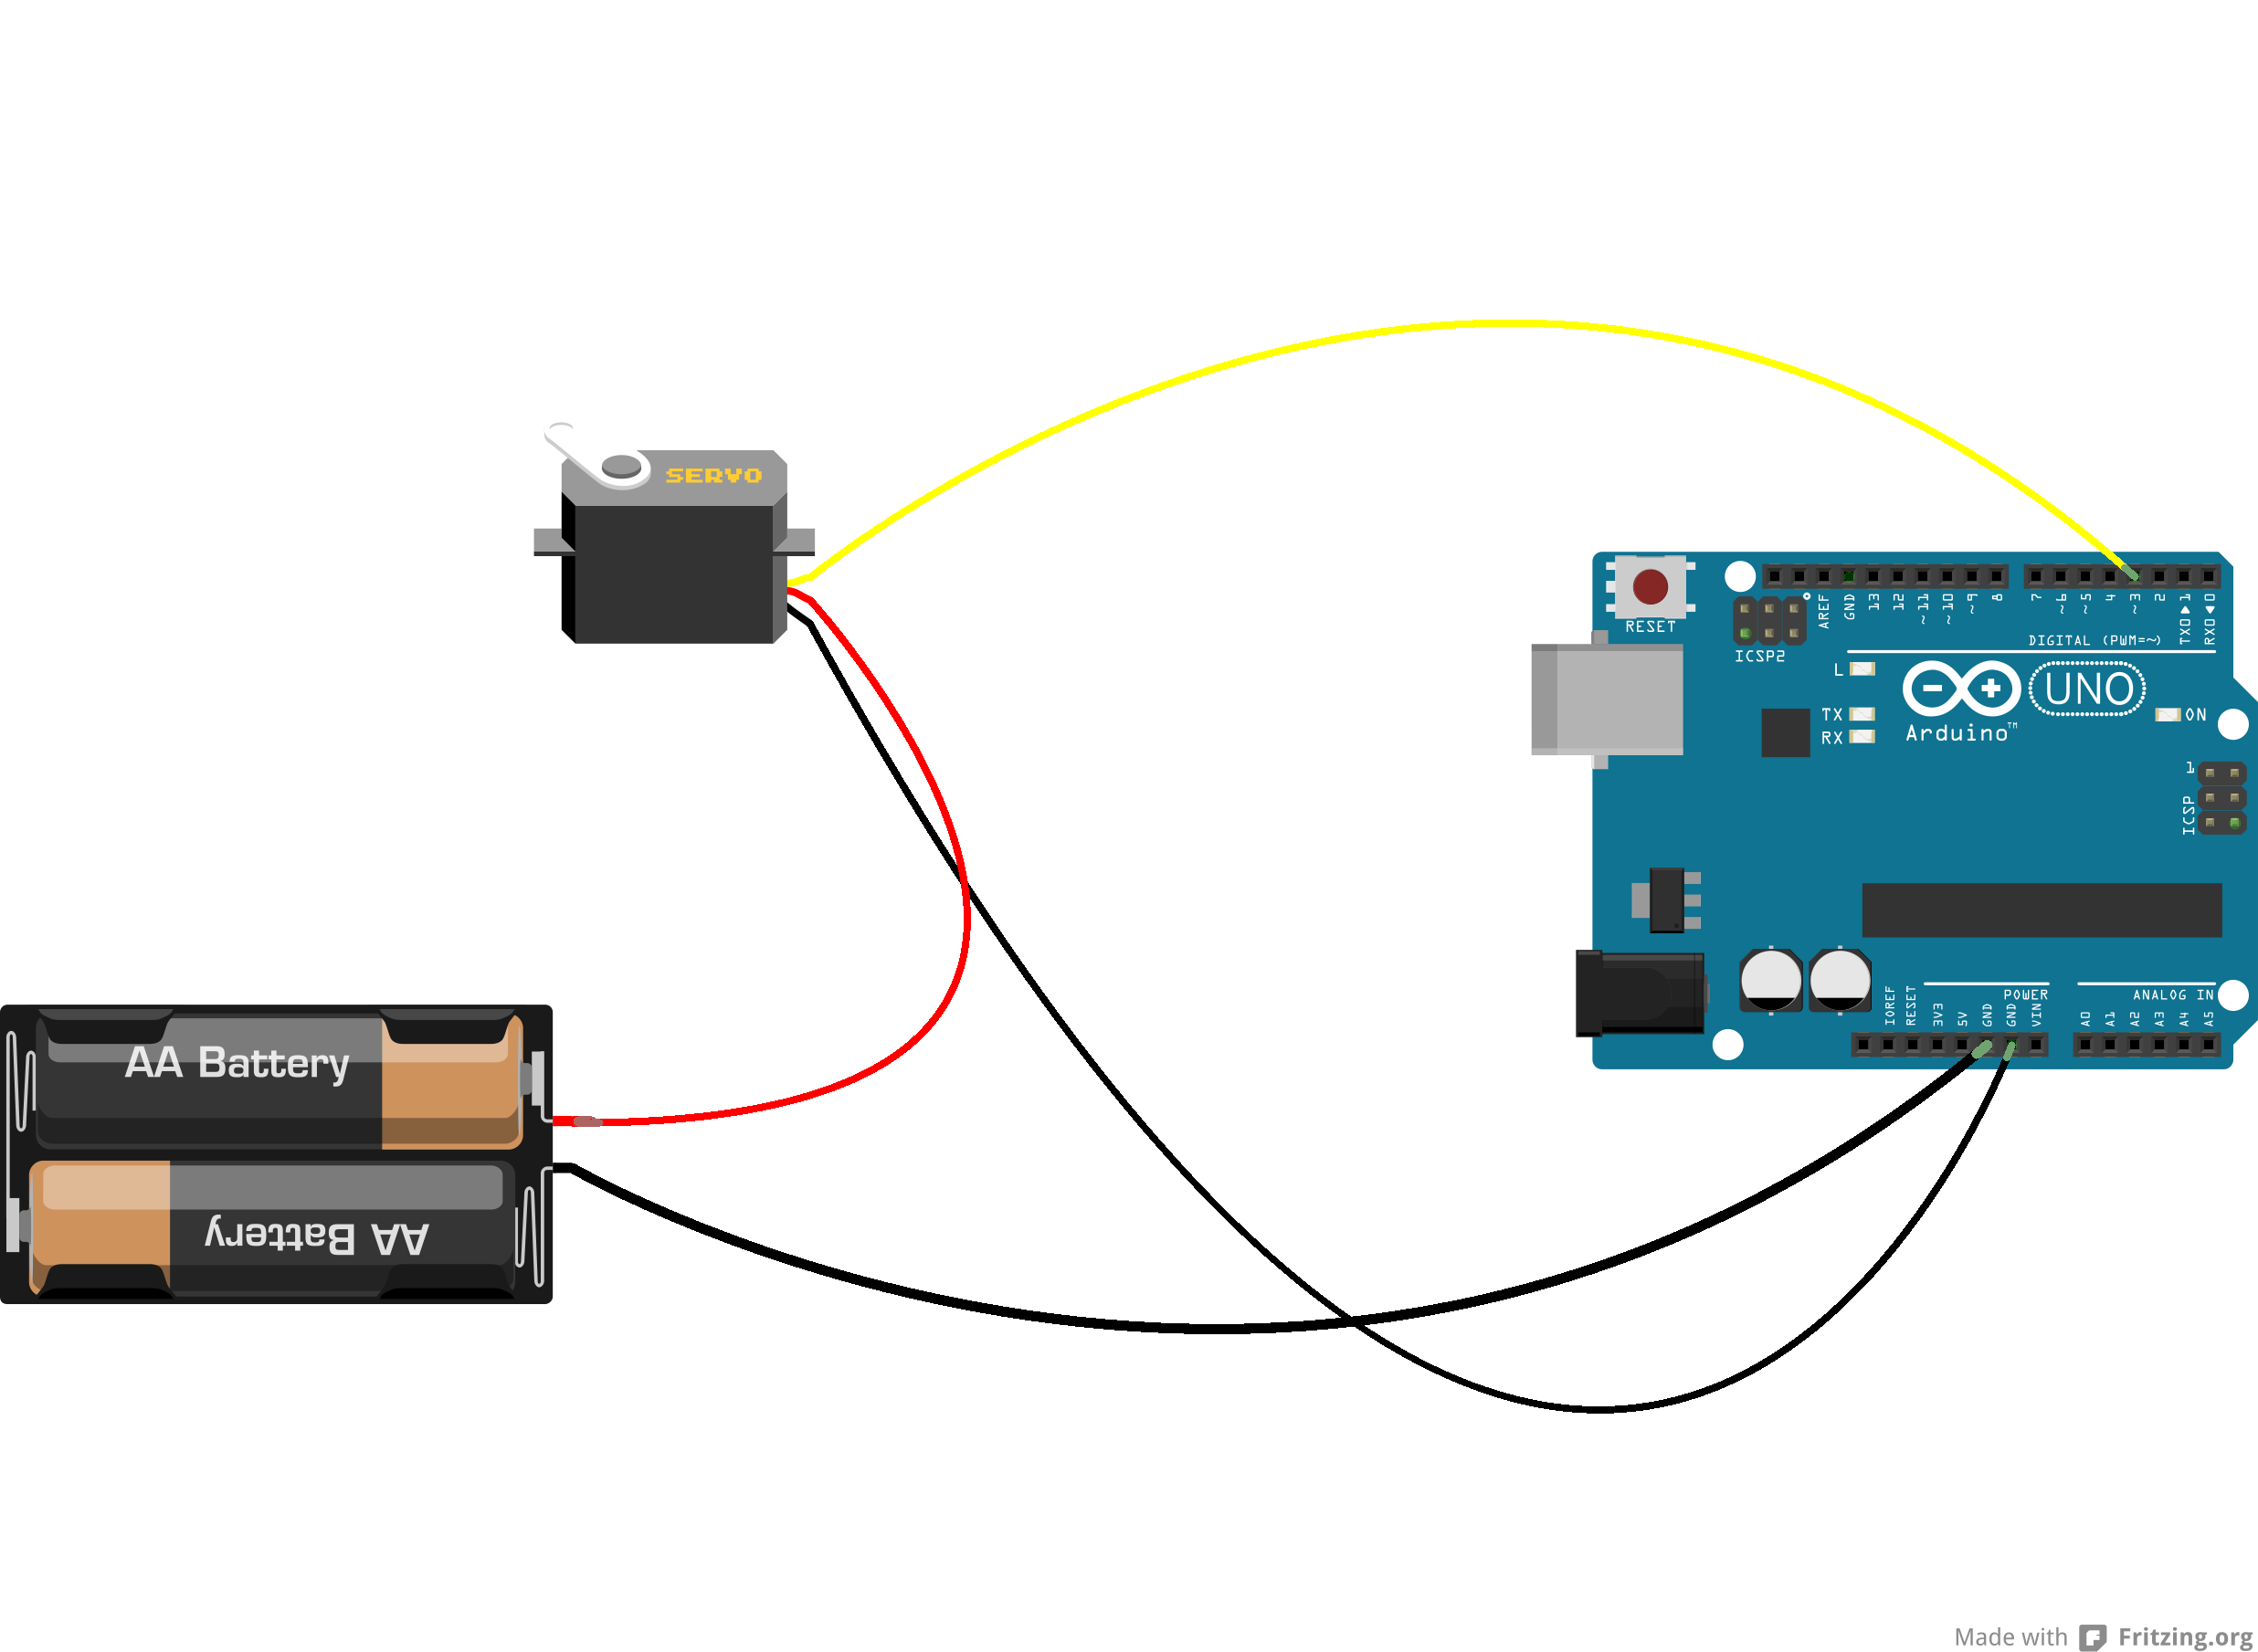
\includegraphics[scale=0.75]{regular_servo.png}
\caption{Connection for Regular Servo motor. Battery represents 5VDC bench supply!}
\label{regularServo}
\end{figure}

If you wish to connect the Servo motor through the LCD shield, refer to blah for the connection mapping


\begin{figure}[ht!]
\centering
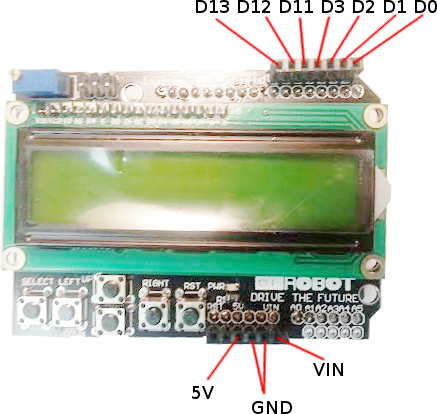
\includegraphics[scale=0.75]{lcd_shield.png}
\caption{Arduino connections mapped through LCD shield}
\label{LCDShield}
\end{figure}

\section{Sending commands to the Servo}

Servo commands are sent as precise digital pulses.



From Wikipedia(http://en.wikipedia.org/wiki/Servo\_control):

``{\em The servo expects to see a pulse every 20 ms, however this can vary within a wide range that differs from servo to servo. The length of the pulse will determine how far the motor turns. For example, a 1.5 ms pulse will make the motor turn to the 90 degree position (neutral position).}''

For our purposes today, we do not need to know exact pulse widths - the Arduino has a Servo library that takes care of that for us.  

\begin{lstlisting}[language=C]
Servo myServo;	//declare a Servo object
myServo.attach(servoPin);	//servoPin is the pin used to send pulses
myServo.write(90);	//move the servo to the 90 degree (neutral) position
\end{lstlisting}

%part 1 - use left/right buttons to move forward, backward

\section{Control position with left/right buttons}


%part 2 - use up/down to adjust step size, display state on LCD


\section{Control step size with up/down buttons}

\end{homeworkProblem}
\clearpage


%----------------------------------------------------------------------------------------
%	Exercise 6
%----------------------------------------------------------------------------------------

\begin{homeworkProblem}[Continuous Servo Motor]

In the hobbyist RC market, the servo protocol is widely used - some remote control receivers output standard servo pulses for all channels, for example.  In some instances, hobbyists want to control a standard motor from these servo commands.  As you have likely found, however, regular servos have a limited rotation range, so to get around this, `continuous rotation' servos have become commercially available.  These typically do not have any speed control - only forwards, backwards, or stop.  In our lab apparatus, we use a continuous rotation servo to control the conveyor belt.

%part 1- move via serial
For part 1, control your continuous rotation servo via serial command.  This is a common technique to control arduino-based hardware from a PC - it is easy to write programs that communicate via USB serial port.


%part 2 - move via LCD interface
Move the continuous rotation servo via LCD interface

%part 3 - move until optical satisfies
Move the continuous rotation servo until the optical sensor becomes obstructed

\end{homeworkProblem}
\clearpage


%----------------------------------------------------------------------------------------
%	Exercise 7
%----------------------------------------------------------------------------------------

\begin{homeworkProblem}[System Integration - Manual Control Mode]


%insert diagram of lab apparatus

In this lab, we will begin interfacing to the lab apparatus.  

The user should be able to:
\li{Use the left/right buttons to move the conveyor belt}
\li{Use the up/down buttons to move the lifter assembly}
\li{use the 'Select' button to push the extruder}

This will allow you to determine timing constants for the various operations required for the full integration in exercise 8

\end{homeworkProblem}
\clearpage


%----------------------------------------------------------------------------------------
%	Exercise 8
%----------------------------------------------------------------------------------------

\begin{homeworkProblem}[System Integration - Automatic Mode]


In automatic mode, the user should be able to push the "Select" button and print {\em at least two} cookies on the tray.  A state machine approach is recommended, and provided partially in the example code.  


Super bonus awesome points: Let the user select the number of cookies to print via the LCD interface... but keep a safety check to ensure the extruder only actuates when there is a tray underneath it!

\end{homeworkProblem}
\clearpage


\end{document}
